\documentclass{beamer}

\usepackage[italian]{babel}
\usepackage[utf8]{inputenc}
\usepackage{graphicx}

\title{Introduzione a \texttt{git}}
\author{Luca Tagliavini, Stefano Volpe}
\institute{Università di Bologna, corso di Laurea in Informatica}
\date{8 novembre 2022}
\logo{
\includegraphics[width=0.05\textwidth]{assets/by-nc-sa-4-0.png}}

\AtBeginSection[]{
  \begin{frame}
    \frametitle{In questa sezione}
    \setcounter{tocdepth}{2}
    \tableofcontents[currentsection]
  \end{frame}
}

\begin{document}

\begin{frame} 
  \titlepage
\end{frame}

\section{Controllo di versione}

\subsection{Problemi}
\begin{frame}{Problemi}
  Quando lavoriamo con molti \emph{file} (redigiamo documenti, creiamo arte
  digitale, scriviamo codice...), ricorrono alcuni \textbf{problemi}:\pause
  \begin{itemize}
    \item<1-> mantenere una \textbf{cronologia} delle modifiche;\pause
    \item<2-> \textbf{ripristinare} subito un qualsiasi stato precedente;\pause
    \item<3-> collaborare a \textbf{copie diverse} dello stesso progetto.\pause
  \end{itemize}
  Copie di cartelle e blocchi note condivisi in rete non bastano più!
\end{frame}

\subsection{Rimedi}
\begin{frame}{Rimedi}
  \begin{definition}
    Un \textbf{sistema per il controllo di versione} (o VCS, \emph{version control
    system}) è un applicativo che gestisce modifiche a grandi insiemi di
    informazioni.
  \end{definition}\pause
  \begin{figure}
    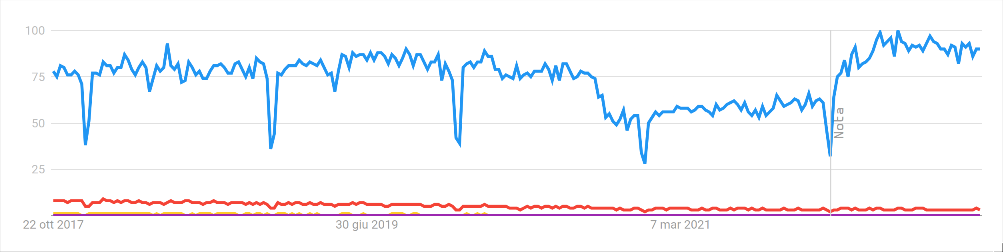
\includegraphics[width=\textwidth]{assets/vcs-popularity.png}
    \caption{popolarità su Google dei cinque principali VCS
    (\textcolor{cyan}{Git}, \textcolor{red}{SVN},
    \textcolor{orange}{Mercurial}, \textcolor{green}{Perforce},
    \textcolor{violet}{CVS}) negli ultimi cinque anni. In ordinata, 100 indica il
    massimo storico del più popolare di questi in tale lasso di tempo.}
  \end{figure}
\end{frame}

\subsection{Ambiente di lavoro}
\begin{frame}{Ambiente di lavoro | Scopo}
  Nei prossimi lucidi, collegandoci alle macchine di laboratorio con i nostri
  utenti, useremo \texttt{git} da linea di comando.\pause
  \begin{block}{Consiglio}
    Tenete aperta questa presentazione anche sulla vostra macchina durante il
    laboratorio: potete trovarla su
    \href{https://csunibo.github.io/lab}{\beamergotobutton{csunibo.github.io/lab}}.
  \end{block}
\end{frame}

\begin{frame}{Ambiente di lavoro | Materiali}
  Materiali:
  \begin{enumerate}
    \item<1->un utente nella rete dipartimentale (es. \texttt{stefano.volpe2});
      \begin{alertblock}{Se siete senza utente...}
        ... (e non avete \texttt{git} neanche sulla vostra macchina), seguite con
        chi siede al vostro fianco.
      \end{alertblock}\pause
    \item<2->un client \texttt{ssh}. Su Linux e macOS è già installato; su
      Windows, se vi manca, c'è
      \href{https://www.chiark.greenend.org.uk/~sgtatham/putty/latest.html}{\beamergotobutton{PuTTY}}.
  \end{enumerate}
\end{frame}

\begin{frame}{Ambiente di lavoro | Preparazione}
  Preparazione:
  \begin{enumerate}
    \item<1->scegliere una delle \href{https://disi.unibo.it/it/dipartimento/servizi-tecnici-e-amministrativi/servizi-informatici/accesso-remoto}{\beamergotobutton{macchine
      di laboratorio}} (es. \texttt{XXX.cs.unibo.it}, dove \texttt{XXX} è il
      nome della macchina scelta)
    \item<2-> collegarsi:
      \begin{semiverbatim}
        \$ ssh stefano.volpe2@XXX.cs.unibo.it
      \end{semiverbatim}
  \end{enumerate}
\end{frame}

\begin{frame}{Ambiente di lavoro | Preparazione (2)}
  \begin{semiverbatim}
  \lbrack ...\rbrack \newline
  Are you sure you want to continue connecting \newline (yes/no/\lbrack
  fingerprint\rbrack)? yes \newline
  \lbrack ...\rbrack \newline
  stefano.volpe2@XXX.cs.unibo.it's password:
  \end{semiverbatim}
\end{frame}

\section{Basi di \texttt{git}}

\subsection{\texttt{git init}}
\begin{frame}
  \frametitle{\texttt{git init}}
\end{frame}

\subsection{\texttt{git add}}
\begin{frame}
  \frametitle{\texttt{git add}}
\end{frame}

\subsection{\texttt{git status, commit}}
\begin{frame}
  \frametitle{\texttt{git status, commit}}
\end{frame}

\subsection{\texttt{git log}}
\begin{frame}
  \frametitle{\texttt{git log}}
\end{frame}

\subsection{\texttt{git branch, checkout, switch}}
\begin{frame}
  \frametitle{\texttt{git branch, checkout, switch}}
\end{frame}

\section{Collaborazione remota}

\subsection{\texttt{git remote}}
\begin{frame}
  \frametitle{\texttt{git remote [show]}}
  Una repository locale pu\`o essere collegata ad una remota per facilitare la
  collaborazione, per la distribuzione del codice o per ragioni di backup.
  La gestione degli endpoint remoti a cui si vuole collegare avviene tramite la
  famiglia di comandi \texttt{git remote}. \\
  Per ottenere una lista di remoti collegati alla nostra repository e delle
  loro propriet\`a si ha il comando:
  \begin{semiverbatim}
  \$ git remote [-v]
  \end{semiverbatim}
  Alternativamente si possono ottenere ancora pi\`u informazioni con il comando:
  \begin{semiverbatim}
  \$ git remote show [name]
  \end{semiverbatim}
\end{frame}

\begin{frame}
  \frametitle{\texttt{git remote add, remove}}
  Per configurare un nuovo remoto per la nostra repository possiamo usare il
  comando:
  \begin{semiverbatim}
  \$ git remote add <name> <uri>
  \end{semiverbatim}
  passando un opportuno \texttt{URI}. L'indirizzo pu\`o essere di tipo
  \texttt{HTTP}, \texttt{SSH} ma anche un percorso sul proprio filesystem
  contenente una opportuna repository. Il nome standard per il remoto principale
  \`e \emph{origin}. Nella maggior parte dei provider moderni l'utilizzo di
  \texttt{HTTP(S)} \`e stato deprecato per ragioni di sicurezza. In questa guida
  useremo sempre remoti con protocollo \texttt{SSH} e voi dovreste fare
  altrettando. \\
  \texttt{remove} \`e il sottocomando speculare ad \texttt{add} che consente di
  rimuovere un remoto dato il nome:
  \begin{semiverbatim}
  \$ git remote remove <name>
  \end{semiverbatim}
\end{frame}

\subsection{\texttt{git push}}
\begin{frame}
  \frametitle{\texttt{git push}}
  Una volta aggiunto un endpoint \`e possibile caricare i propri commit alla
  repository remota:
  \begin{semiverbatim}
  \$ git push [-u] [<name>]
  \end{semiverbatim}
  Dover specificare il nome del remoto ogni volta pu\`o diventare tedioso, di
  conseguenza \`e tipico configurare un remoto predefinito, denominato
  \emph{upstream}, eseguendo un \texttt{push} con la flag \texttt{-u}. \\
  % TODO: mhhh
  Nel tempo si \`e esteso il significato del termine \emph{upstream} per
  indicare la repository "originale" nel contesto fork tra progetti.
\end{frame}

\subsection{\texttt{git fetch, pull}}
\begin{frame}
  \frametitle{\texttt{git fetch, pull}}
\end{frame}

\subsection{\texttt{git merge}}
\begin{frame}
  \frametitle{\texttt{git merge}}
\end{frame}

\end{document}
